\chapter{Multimodal Black-box Models}
\label{chapter:multiodality}

\textit{"Learning is lifelong; we forget rules when they no longer apply or revise them when the environment changes."} - Ethem Alpaydin 

\section{Chapter Overview}
In the previous chapter, we used only CNVs, i.e., single modality to develop a decision support system~(DSS). It was based on snapshot neural ensemble method of two independent deep architectures called \texttt{Conv-LSTM} and \texttt{CAE} networks. Eventhough, it was technically a black-box model, the DSS performed moderately well at predicting cancer types. As discussed earlier that to develop a more reliable and accurate DSS for cancer diagnosis, multiple factors have to be considered. In this chapter, the single modality-based DSS is extended to multimodality. A multimodal autoencoder~(MAE) classifier is trained on genomics data to classify breast cancer patients based on the presence of PGR, ER, and HER/2 neu statuses\footnote{\textbf{RQ1}: How to use multimodal genomic data to accurately predict cancer
types?}. Effects of different modalities are observed and assess the performance of our CDSS across breast cancer subtype classification. The idea is based on the hypothesis\footnote{\textbf{H3}: Multimodal genomics data and clinical outcome can be used to train a multimodal neural network architecture to provide more accurate clinical diagnostic decision.} that multimodal genomics data and clinical outcome can be used to train the MAE architecture to provide more accurate clinical diagnostic decision\footnote{\textbf{Supporting publication}: \textbf{Md. Rezaul Karim}, Stefan Decker, Oya Beyan, ``Multimodal Autoencoders for Prognostically Relevant Subtypes and Survival Prediction for Breast Cancer", \emph{IEEE Access}, DOI: 10.1109/ACCESS.2019.2941796, September 2019.}. 

\section{Introduction}
\label{secIntroduction_Motivation}
Accurate diagnosis and prognosis to cancer are specific to patients with particular cancer subtypes and molecular traits. For example, diagnosis and subsequent treatments for breast cancer patients depends on distinct molecular subtypes such as `Luminal A', `Luminal B', `HER2-enriched', and `Triple-negative'~(TN)~\cite{sorlie,dai}. `Luminal A' patients generally requires only endocrine therapy. On the other hand, chemotherapy is considered necessary for the `Luminal B', `HER2-enriched', and `Triple-negative' patients~\cite{goldhirsch}. Besides, breast cancer characterize by ER, PGR, and HER2, represents a subset of breast cancer with different biologic behavior: ER, PGR, and HER2 statuses are mainly involved in determining breast cancer subtypes. %and survival rates. 
Further, breast cancer patients can be categorized into ER `POSITIVE', `NEGATIVE', or `INDETERMINATE' in which ER negative tumors are associated with a worse clinical outcome compared to ER-positives~\cite{karimACCA2019}. 

\hspace*{3.5mm} Therefore, knowing the subtypes of a breast cancer patient is prerequisite before recommending the best possible treatment. The cancer sub-typing task involves: i) learning useful and distinctive biological features from a set of genomic input modalities, and ii) and using machine learning~(ML) techniques to classify similar patients that share similar biological characteristics. Although tree-based ensemble such as random forest and gradient boosting trees are widely used at variety tasks, they are not suitable for handling multiple input modalities. Given they only able to learn from the intersection of samples, which are both clean and labeled. Major advantage of DNN-based joint representations comes from their often superior performance and the ability to pre-train the representations in an unsupervised manner. 

\hspace*{3.5mm} A well-trained model is subject to enough data as DNNs require a lot of labeled training data. The multilayer nature in DNN and it's successive layer is hypothesized to represent the data in a more abstract way~\cite{mmsurvey}. Each modality starts with several individual neural layers followed by a hidden layer that projects the modalities into a joint space~\cite{serban2016multi}. It is common to capture the output of the deepest layer as a form of data representation from individual modalities~\cite{mmsurvey,serban2016multi}. For example, breast cancer patients can be broadly categorized into different groups depending upon the presence and involvement of estrogen receptor~(ER), progesterone receptor~(PGR), and human epidermal growth factor receptor 2~(HER2/neu protein in normal cell growth. Since CNV data does not cover these biomarkers of the patient, providing AI-based diagnoses solely based on CNV might not be accurate and reliable. Nevertheless, our real world experience is multimodal~\cite{mmsurvey}, e.g., while watching a movie, we not only observe the movie itself, but also the acting, background music, action sequences, background scenario, and landscapes, etc. Similarly, the multimodal machine learning~(ML) aims to build a ML model capable of processing and relating information from multiple modalities~\cite{mmsurvey}. 

\hspace*{3.5mm} Multimodal representation learning generates distributed vectors by mapping multiple modalities of information to a single mathematical space, where the similarities are attributed based on a distance measure. A unimodal representation technique is sufficient for each respective modality in the multimodal space~\cite{ito2018effects}. Cheerla et al.~\cite{cheerla2019deep} and Phan et al.~\cite{phan2016integration} have exposed that cancer diagnosis based on multimodal data is both clinically and biologically effective and accurate. A multimodal genomics dataset can be prepared to perform multimodal representation learning, by: i) combining DNA methylation, gene expression~(GE), and miRNA expression from different cohorts, ii) creating a multiplatform network to support each modality. 

\hspace*{3.5mm} The joint multimodal representation is then passed through multiple hidden layers itself or used directly for prediction. A multimodal neural network can be trained end-to-end to represent the data to perform both supervised and unsupervised tasks. In such a network topology, multimodal representation and multimodal fusion are learned together~\cite{wang2018associativemulti}. Performance of a conventional unimodal information fusion architecture is greatly affected by its ability to detect and combine useful and complementary information from heterogeneous representations stemming from a set of distinctive modalities~\cite{ito2018effects}. However, one of the disadvantages comes from the model not being able to handle missing data, which is mainly due to the reconstruction losses during the pre-training goes unbound. Therefore, it is common to pre-train such representations using an autoencoder on unsupervised data~\cite{mmsurvey}. 

\hspace*{3.5mm} Multimodal information fusion is the concept of integrating information from multiple modalities with the goal of predicting an outcome measure~\cite{mmsurvey,mmdcae}. Multimodal fusion provides three main benefits over unimodal learning~\cite{mmsurvey}: i) having access to multiple modalities that observe the same phenomenon may allow for more robust predictions, making the clinical DSS more reliable, ii) having access to multiple modalities might allow us to capture complementary information, e.g., we can often integrate genomics, proteomics, bioimaging, texts, or even clinical outcomes to support each other, iii) a multimodal system can still operate when one of the modalities is missing, e.g., in case of missing bioimaging, we can still rely on genomics, proteomics, and clinical outcomes.

%In multimodal fusion learning, multimodal perspectives is required to together~\cite{mmsurvey}. 
\hspace*{3.5mm} From biological perspective, it is analogous to create knowledge together from multimodal perspectives in a way humans can understand~\cite{mmdcae}. Since each type of data has different intrinsic statistical features, they cannot be compared in a trivial way. The rest of the chapter is structured as follows: \cref{chapter_4:rw} covers related works concerning cancer diagnosis based on multimodality data and summarize their potential limitations. \Cref{chapter_4:mm} describes the overall approach, including the detail of the data collection and feature engineering before the network construction and training. \Cref{chapter_4:results} demonstrates the experiment results. \Cref{chapter_4:discussion}, discusses key findings of the study. \Cref{chapter_4:conclusion} provides some explanations of the importance and relevance of the study reported, highlights the limitations and discuss some future works. % before concluding the chapter. 

\section{Related Work}\label{chapter_4:rw}
Even a few years ago, most popular approaches for graphical-model based representation are deep Boltzmann machines~(DBM), that stack restricted Boltzmann machines~(RBM) as building blocks. Similar to DNNs, each successive layer of a DBM is expected to represent the data at a higher level of abstraction. The appeal of DBMs comes from the fact that they do not need supervised data for training. As they are graphical models the representation of data is probabilistic, however it is possible to convert them to a deterministic DNNs, which, however, loses the generative aspect of the model. Although, approaches using both unimodal~\cite{abdel2016breast} and multimodal DBN~\cite{liang} show accuracy at different prediction tasks, one of the potential limitations using DBN-based approaches is that the limited capability at feature learning during pretraining~\cite{serban2016multi}, although it gets a decent set of feature representations for the inputs. Furthermore, DBN is incapable of learning quality features from very high dimensional datasets. Besides, pretraining losses often get out of bound, which results in overfitting issue. 

\hspace*{3.5mm} To overcome the limitations of existing approaches, majority of the multimodal methods focused on representation fusions~\cite{ito2018effects}, either by combining representations before the classification called feature level fusion or by combining the results of classifications performed in single-mode representations in another analysis  called `decision level fusion'~\cite{atrey2010multimodal}. 
The multimodal autoencoder~(MAE) proposed by Ngiam et al.~\cite{NgiamKKNLN11} extended the idea of using autoencoders in the multimodal information fusion setting. They used stacked denoising autoencoders to represent each modality individually and then fused them into a multimodal representation using another autoencoder layer~\cite{mmsurvey,serban2016multi}. It is also common to fine-tune the resulting representation on a supervised learning tasks. 
MAE~\cite{liu2016multimodal,serban2016multi,wang2018associativemulti} can be used to flexibly learn from prior distribution and to capture features from a target distribution. Subsequently, MAE-based approaches have been applied in natural language understanding like tasks such as document and dialogue modeling~\cite{serban2016multi}, emotion recognition~\cite{liu2016multimodal}, and multimodal word representation~\cite{wang2018associativemulti}. 

\hspace*{3.5mm} An alternative to a joint multimodal representation is a coordinated representation, where instead of projecting the modalities together into a joint space, separate representations for each modality are learned but coordinated them through a constraint. Although, there a few recent multimodal approaches for more optimized representation learning, a vanilla autoencoder-based MAE architecture is constructed. Multimodal system presented in~\cite{wang2018associativemulti} is extended by adding the capability of handling multiple modalities across four different types of genomics data. During the multimodal fusion approach, small part of patient data is discarded that don't have all modalities in our MAE network. A fully connected layer is then added for the supervised learning task, i.e. breast cancer subtypes predictions. 

%To provide more reliable cancer identification, 
%and the decision about survival
%several modalities consisting of masked somatic mutations, copy number segment~(CNS) and mask CNS, DNA methylation, GE, miRNA expression along with clinical outcomes were used, instead of a single modality.

\section{Methods}\label{chapter_4:mm}
In this section, we discuss our approach in detail, including data collection, preprocessing, network construction, and training. 

\subsection{Problem statement}
The problem of cancer sub-typing is to observe which genetic mutations are responsible for which breast cancer subtypes, based on multimodal genomics data containing ER, PGR, and HER2/neu statuses of breast cancer patients, either separately or in a multimodal way. 
The heterogeneity of expression across samples is captured in a gene regulation space, instead of gene expression space. This also involves transforming gene expression, miRNA expression, and DNA methylation profiles into regulation profiles for characterizing differential expression of genes between different subtypes. Since breast cancer subtype classification consists of following three sub-tasks based on ER, PGR, and HER2/neu status, each of these will correspond to different neural networks: 

\begin{itemize}
    \item \textbf{ER status classification} - diagnosing individual patients into one of POSITIVE, NEGATIVE, and INDETERMINATE\footnote{Patients can't be grouped as positive, negative, or equivocal}, based on existence of ER protein breast tissue. 
    \item \textbf{PGR status classification} - diagnosing individual patients into one of POSITIVE, NEGATIVE, and INDETERMINATE, based on existence of PGR protein in breast tissue. 
    \item \textbf{HER2/neu status classification} - diagnosing individual patients into one of `POSITIVE, NEGATIVE, INDETERMINATE, and EQUIVOCAL\footnote{Assessments without information on how to treat a patient}, based on existence of HER2 protein in breast tissue. Unlike ER and PGR status, HER2/neu is the most important prognostic biomarkers. 
\end{itemize}

\subsection{Datasets}
\label{dc}
Several databases of genomics data exist including TCGA~\cite{tcga}, ICGC~\cite{icgc}, and COSMIC~\cite{forbes}. Based on public availability and amount of data~(w.r.t. number of patients data), the breast invasive carcinoma~(BRCA) branch of TCGA was considered as the main data source\footnote{TCGA has 39 projects for 39 different cancer types~(v89)}. Clinical data and biospecimens are collected through the Genomics Data Commons~(GDC) data portal\footnote{\url{https://portal.gdc.cancer.gov/}}. Clinical data comprise of general clinical information as well as cancer status~(e.g., cancer location, cancer stage). Besides, some data came in different formats. For example, $70\%$ of the DNA methylation data came from a different platform than the remaining $30\%$, having two structures. It is to be noted that several factors refrained us from using each type of data, e.g., masked somatic mutation data are the base pair~(BP) position in a chromosome, making not all the mutations are significant. 

\begin{figure*}
  \centering
  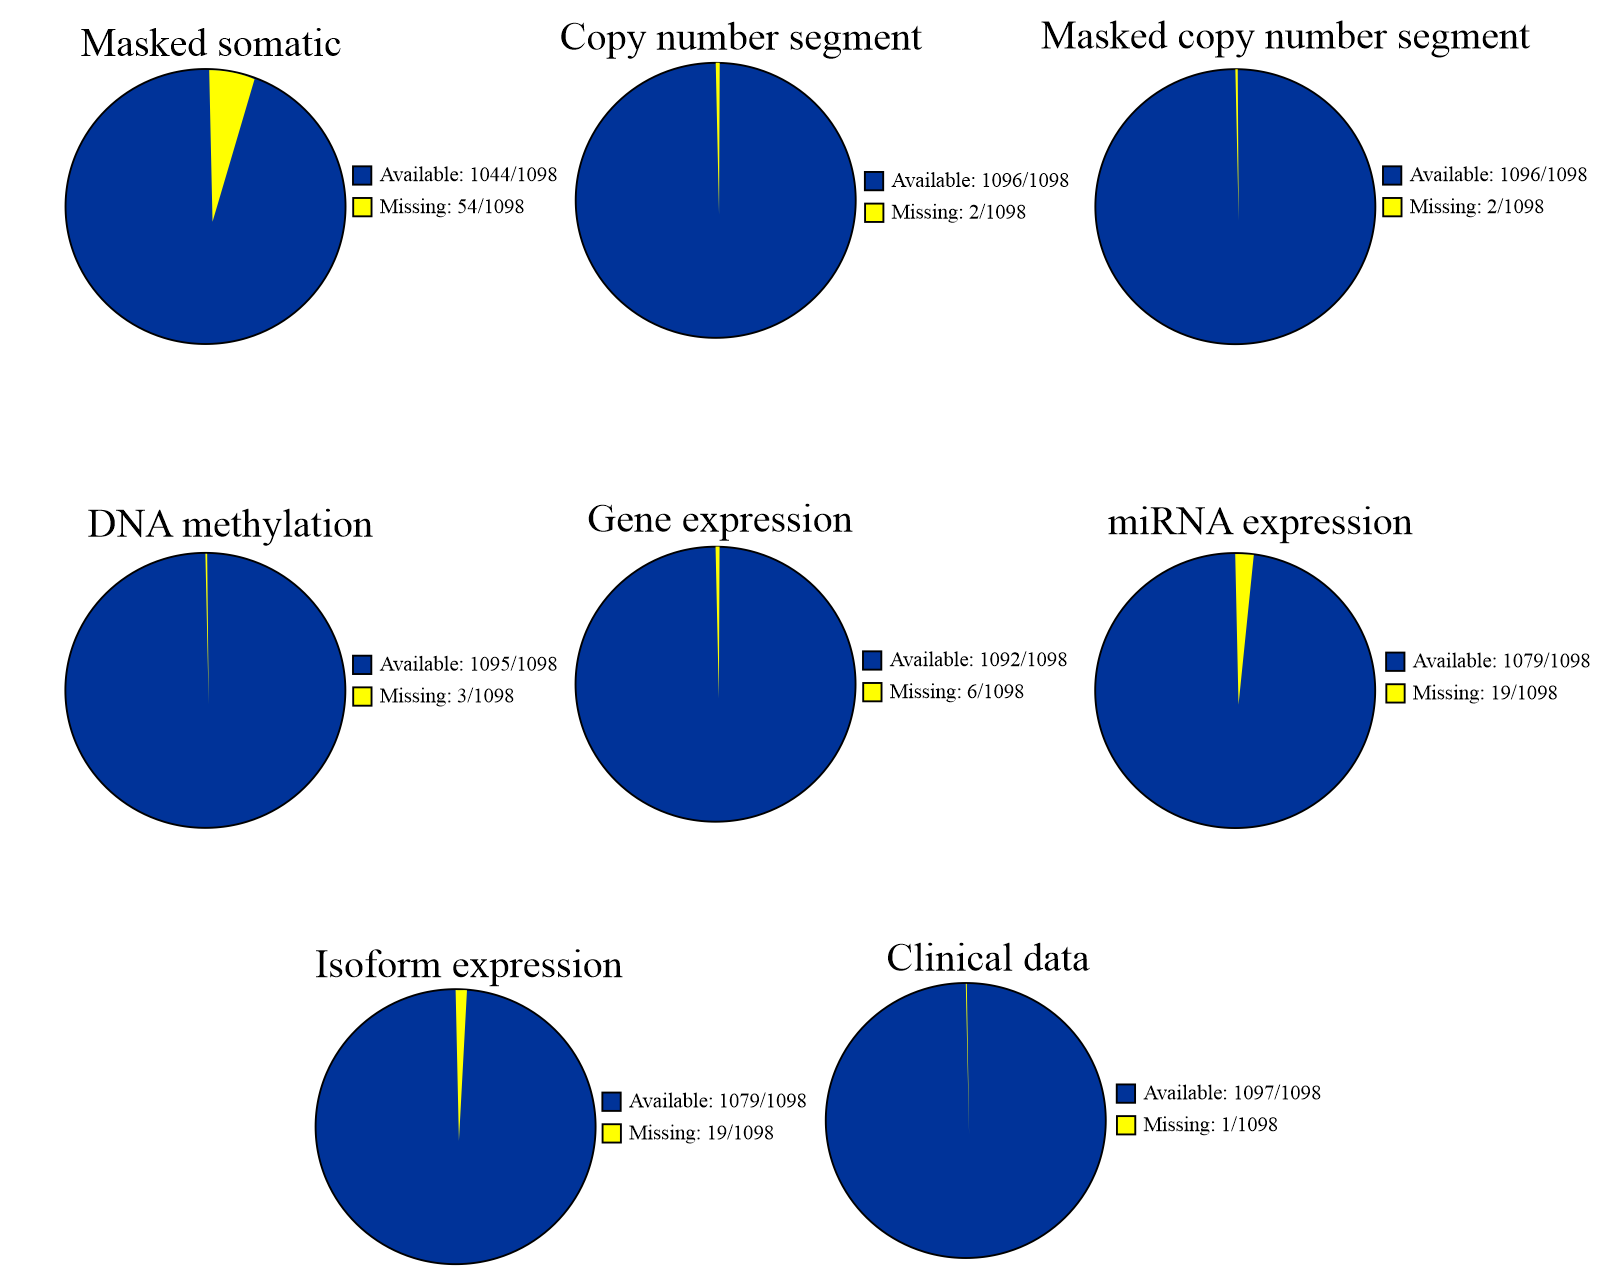
\includegraphics[scale=0.55]{images/data_per_patients}
  \caption[Selection and formation of multimodal breast cancer patient cohorts]{Selection and formation of multimodal breast cancer patient cohorts, where out of 1,098 breast cancer cohorts only 1,000 patients  contribute to multimodal data }
  \label{fig:data_per_patients}
\end{figure*}

\hspace*{3.5mm} CNS and masked CNS were not used because of extremely high dimension and variable structure~(in fact, there was no fixed dimension for each data per patient). Since BP's start refers observed, CNS data and stop positions in a chromosome, which will always vary at a BP resolution. We do not use here copy number and DNA variation gave the extremely high dimension and complex structure of the data, i.e., variant position, will always vary at a base pair resolution. Since GE quantification data covers the amount of RNA synthesized by each gene on a single time, we treat each data per row and consider if the gene's Ensembl ID belongs to the data release. miRNA and GE quantification data from TCGA were already in the desired format, so no preprocessing was required. From the masked somatic data, gene data containing both the Ensembl ID and Hugo gene symbol considered only. 

\hspace*{3.5mm} Both CNS and masked CNS data cover entire gene mutation cases on base-pair sequences instead of a single BP case, which was covered in masked somatic data. Therefore, we find corresponding Ensembl gene ID from the chromosome position and extract the data using Ensembl API~\cite{yates}. Processing DNA methylation data was a complex task due to different platform. In particular, some patients were measured with the HumanMethylation27 platform, while the remaining patients were measured with HumanMethylation450 arrays. Only 26K DNA methylation sites were common in both platforms. With above considerations, gene expression, miRNA expression, and DNA methylation data along with clinical outcomes~(w.r.t pathology responses) are used. 

\begin{table}[h]
    \scriptsize
    \caption{Statistics of the data used for breast cancer sub-type classification~\cite{karimACCESS2019}}
    	\vspace{-2mm}
    \label{tab:all_data_brca}
    \centering
    \begin{tabular}{l|l|l|l} 

        \hline
        \textbf{Tasks}   & \textbf{Input modality} & \textbf{\#Sample } & \textbf{\#Features}  \\ 
        \hline
             & DNA methylation  & 1,046  & 25,978  \\ 
        \cline{2-4}
               & Gene expression   & 1,042 & 60,483      \\ 
        \cline{2-4}
        ER status classification       & miRNA expression                           & 1,029                & 1,881       \\ 
        \cline{2-4}
                                       & Gene + miRNA expression                   & 1,024                & 62,364      \\ 
        \cline{2-4}
                                       & Gene + miRNA expression + DNA methylation & 1,022                & 88,342      \\ 
        \hline
                                       & DNA methylation                           & 1,045                & 25,978      \\ 
        \cline{2-4}
                                       & Gene expression                           & 1,041                & 60,483      \\ 
        \cline{2-4}
        PGR status classification      & miRNA expression                           & 1,028                & 1,881       \\ 
        \cline{2-4}
                                       & Gene + miRNA expression                   & 1,023                & 62,364      \\ 
        \cline{2-4}
                                       & Gene + miRNA expression + DNA methylation & 1,021                & 88,342      \\ 
        \hline
                                       & DNA methylation                           & 917                  & 25,978      \\ 
        \cline{2-4}
                                       & Gene expression                           & 913                  & 60,483      \\ 
        \cline{2-4}
        HER2/neu status classification & miRNA expression                           & 902                  & 1,881       \\ 
        \cline{2-4}
                                       & Gene + miRNA expression                   & 897                  & 62,364      \\ 
        \cline{2-4}
                                       & Gene + miRNA expression + DNA methylation & 895                  & 88,342      \\ 
        \hline
        \iffalse
                                       & DNA methylation                           & 1,082                & 25,978      \\ 
        \cline{2-4}
                                       & Gene expression                           & 1,077                & 60,483      \\ 
        \cline{2-4}
        
        Survival prediction            & miRNA expression                           & 1,064                & 1,881       \\ 
        \cline{2-4}
                                       & Gene + miRNA expression                   & 1,058                & 62,364      \\ 
        \cline{2-4}
                                       & Gene + miRNA expression + DNA methylation & 1,056                & 88,342      \\ 
        \hline
        \multicolumn{1}{l}{}           & \multicolumn{1}{l}{}                      & \multicolumn{1}{l}{} &  
        \fi 
    \end{tabular}
    	\vspace{-4mm}
\end{table}

\hspace*{3.5mm} These data are very high-dimensional, e.g., GE data for each patient, which is structured based on gene id reaches around 60,000 types. A predictor based on GE comes with 60,000 different features. \Cref{tab:all_data_brca} shows the statistics of the preprocessed data for each modality. We find corresponding Ensembl gene IDs from the chromosome position based on GDC API. The samples having the latest gene Ensembl IDs from release 89 are only considered valid. Clinical data covers clinical outcomes of cancer patient treated as general, pathology, treatments, and surgery. We categorized each patient data into different groups, but only the pathology response from the whole clinical outcomes are used. 

\hspace*{3.5mm} Out of all 1,098 breast cancer patients, majority types contribute to 1,000, by discarding the rest. Following seven different modalities\footnote{Last two modalities were used for the training and evaluation but not reported due to low accuracies.} are subsequently formed. In other words, the training sets are formed from any combinations of DNA methylation, GE, and miRNA expression data, as shown in \cref{fig:data_per_patients}. Besides, some preprocessed data were reused\footnote{Based on a Master thesis I co-supervised with Dr. Oya Beyan: "Analysis of Breast Cancer Genomic Data with Multimodal Deep Belief Network", by Galih Wicaksono, Software Systems Engineering, RWTH Aachen University, 2018}. Based on above consideration, the input to the network can be a single or multimodality in combination with DNA methylation, GE, or miRNA expression data, as shown in. Single type input is considered with a regular AE and multiple types of input with an MAE. For both ER, PGR, and HER2/neu-based sub-type classification are done based on both unimodal inputs with a regular AE and multimodal input with MAE. 

\iffalse
\begin{enumerate}[noitemsep]
    \item DNA methylation 
    \item Gene expression 
    \item miRNA expression 
    \item Gene expression + miRNA expression 
    \item Gene expression + DNA methylation 
    \item miRNA expression + DNA methylation  
    \item DNA methylation + gene expression + miRNA expression. 
\end{enumerate}
\fi 

\begin{figure*}
	\centering
	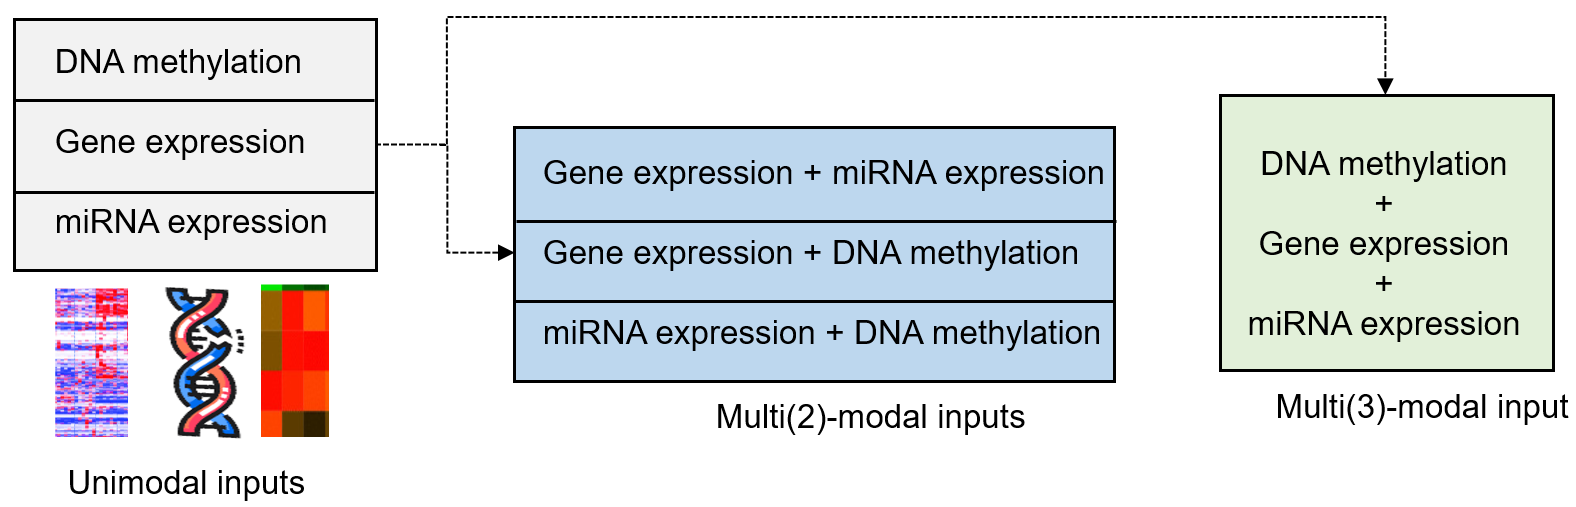
\includegraphics[scale=0.7]{images/input_combination.png}
	\caption[Different uni- and multi-modality input combination]{Unimodal and multimodal input combination with DNA methylation, GE, or miRNA expression}
	\label{fig:input_comb}
\end{figure*}

\subsection{Network construction and training}
Although a single and simple AE can be used to reconstruct an output similar to the original input, it cannot handle multimodality~(i.e., different types of information). In contrast, weights of the MAE encoder learn from both clean, unsupervised data with no labels, and noisy supervised data with missing modalities, leveraging as much of the available data as possible.
Nevertheless, difference w.r.t dimensionality among modalities are pretty large. For example, GE data come with about 60,000 features, but miRNA has only 1,800 features. This non-trivial challenge in modality specific representation learning is enough motivation towards multimodal representation learning and classification, given that an individual latent representation is require to have the same dimensionality~\cite{mmdcae}.

%\subsubsection{Network construction}
\hspace*{3.5mm} The MAE architecture depicted in \cref{fig:slr_1} is used to generate the shared representation for all input modalities, instead of one latent representation for each input modality. \Cref{fig:input_comb} shows the different input modality combination considered, while \cref{tab:all_data_brca} gives the sample distributions. From network topological point of view, MAE creates hierarchical hidden units, which have strong connections between nodes not only for individual modality, but also across the modalities.  
%\subsubsection{Network training}
Training MAE involves pre-training to leverage the learning representation, followed by supervised fine-tuning for the classification based on learned  representation from the multimodal input features. 

\begin{sidewaysfigure*}
	\centering
	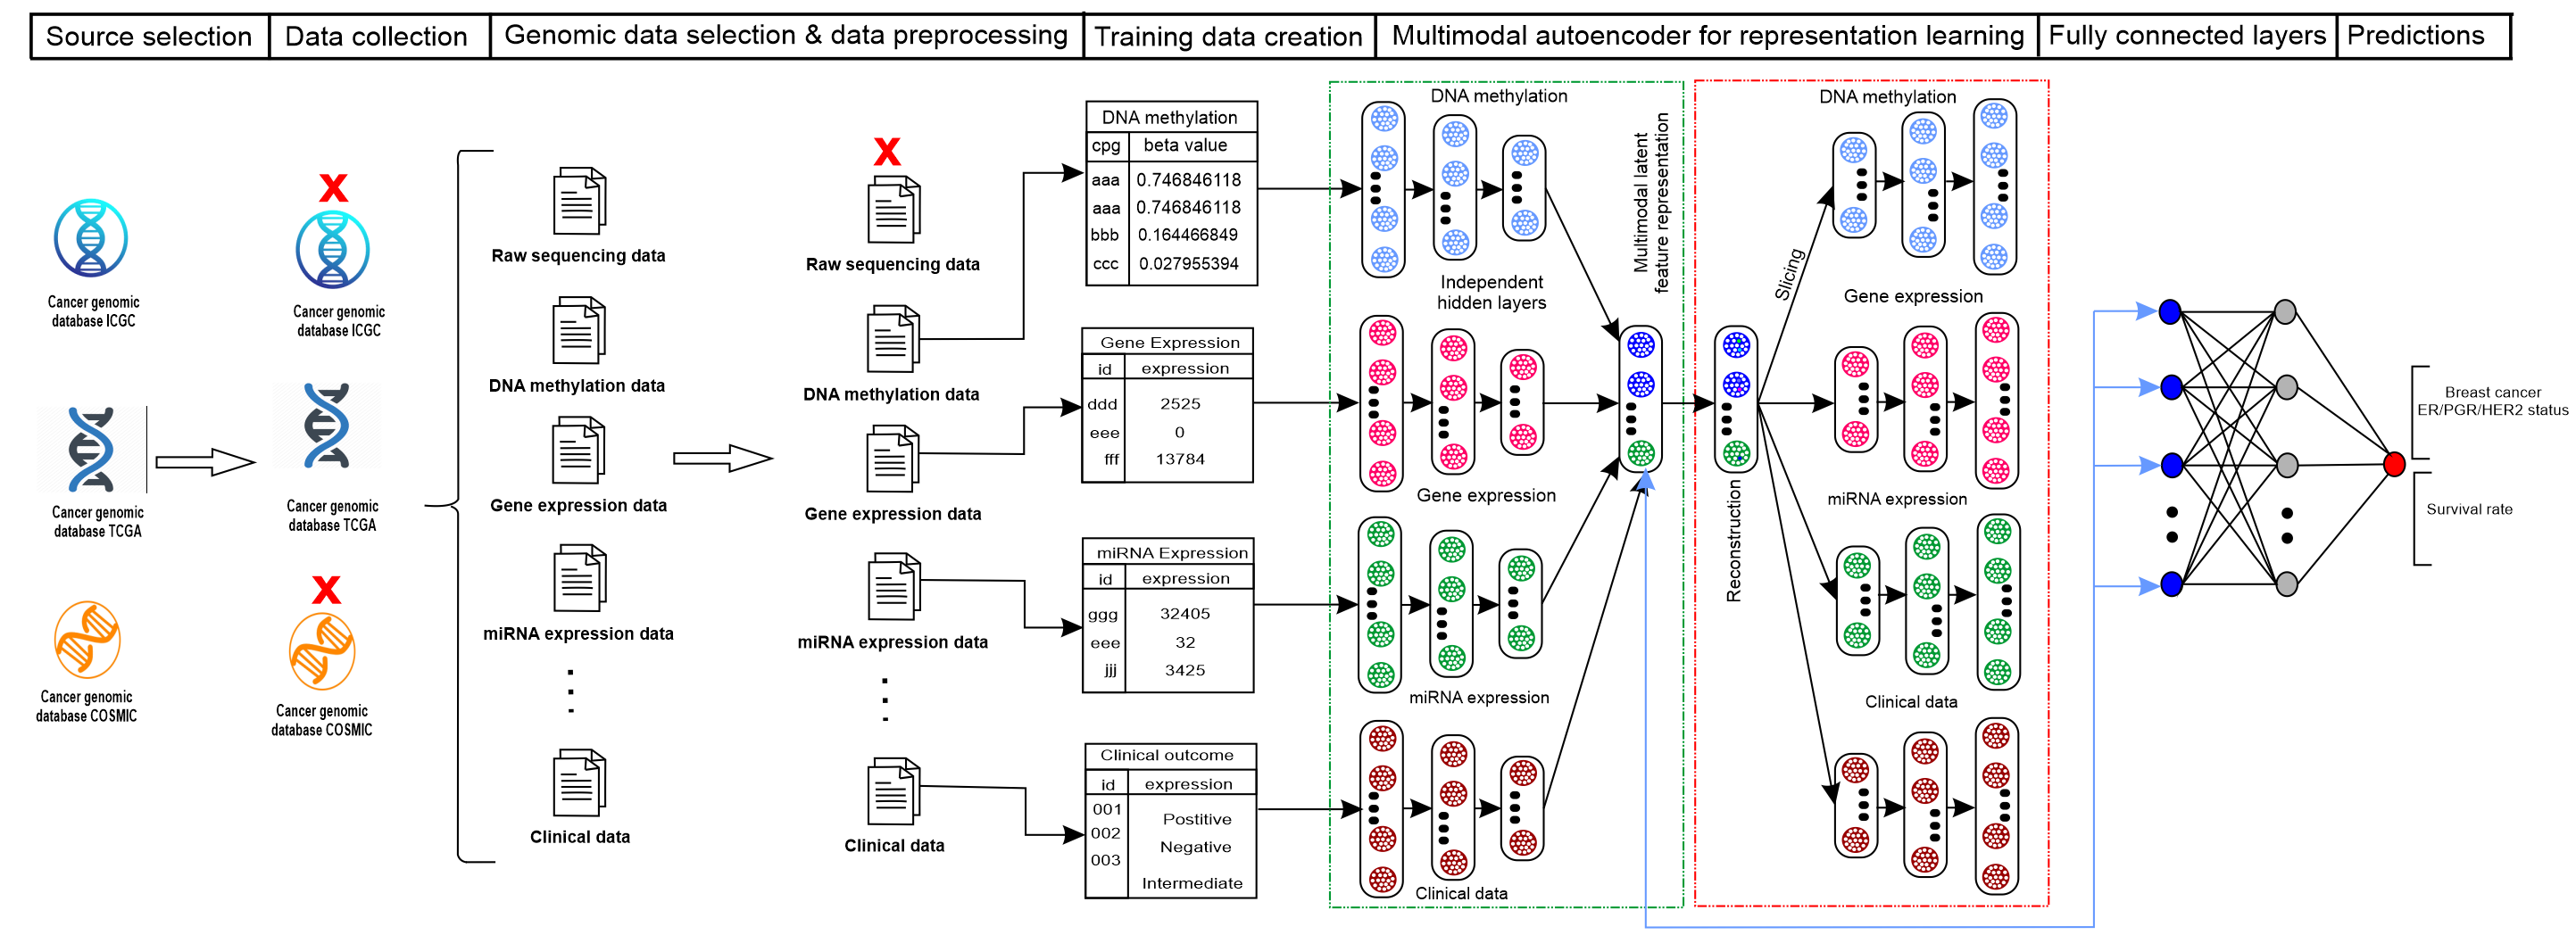
\includegraphics[scale=0.75]{images/mae_v2.png}
	\caption[Workflow of the multimodal autoencoder classifier]{Workflow of the multimodal autoencoder-based classifier in which same input types with different features for subtypes %and survivals 
	are used~\cite{karimACCESS2019}}
	\label{fig:wf_mae}
\end{sidewaysfigure*}

\subsubsection{Unsupervised pre-training} 
Pre-training is similar to training a two-stage AE network: first stage represents modality specific learning. The second stage corresponds to cross-modality. 
%Once the unimodal and cross-modal stages are constructed, training both stages is similar to unsupervised pre-training of the whole MAE architecture.
Pre-training is performed greedily on each layer of the network, which corresponds to representation learning with individual AEs. 

\paragraph{Stage-1: individual modality}\noindent of the MAE represents a particular modality for each type of data. Individual modality AE is not only a one-layer AE, but also a multilayer and gradually shrinking AE with different number of layers per modality. An AE consist of two sub-networks called encoder and decoder. Encoder is a sigmoid function $g(.)$ parameterized by $\phi$, while decoder function $f(.)$ is   parameterized by $\theta$ is an identify function. For input $X_{k} \in \mathbb{R}^{D}$ for each of $k \in \mathbb{R}^K$ modalities, the encoder encodes the original high-dimension input into a lower-dimensional code, where the input size is larger than the output size. Latent-space representation $Z_k=g_{\phi}(X_{k})$ is then learned in the bottleneck layer such that $X_{k}$ is mapped and transformed into embedding space~($Z_k$), where $p$ and $n$ is number of hidden and input units~\cite{mmdcae}: 

\begin{equation}
    Z_k = h_{k}=g_\phi \left({X}_{k}\right)=\sigma\left(W_{k} X_{k}+b_{k}\right)
\end{equation}

\iffalse
\hspace*{3.5mm} For input $X_{k} \in \mathbb{R}^{D}$ for each of $k \in \mathbb{R}^K$ input modalities, encoder function $g_{\phi{k}}$ learns the representation of $X_{k}$ in a compressed form, where the input space is mapped and transformed into an embedding space~\cite{mmdcae}. Let $p$ and $n$ denote the number of hidden and input units in the encoder, respectively: 

\begin{equation}
    h_{k}=f_\theta \left({X}_{k}\right)=\sigma\left(W_{k} X_{k}+b_{k}\right)
\end{equation}
\fi 

\hspace*{3.5mm} where $\phi$ are trainable parameters, which includes the weight matrix $W_{k} \in \mathbb{R}^{n \times p}$ and the bias vector $b_{k} \in \mathbb{R}^{n}$ that are specific to respective modality $k$, and $\sigma$ is the $ReLU$ activation function. The decoder tries to reconstruct from $h_k$, the original input $X_{k}$ from the latent space representation $Z_k$ using function $f(.)$. That means, the hidden representation $h_{k}$ is then mapped back by the decoder function to reconstruct $\hat{X}_{k}$, similar to original input ${X}_{k}$, giving the following reconstructed version of the original input:

\begin{equation}
    \hat{X_k}=f_{\theta}\left(Z_k\right)=f_{\theta}\left(g_{\phi}({X_k})\right). 
\end{equation}

\begin{equation}
    \hat{X_k}=\Psi \left(\hat W_k h_k + \hat b_{k}\right)
\end{equation}

\hspace*{3.5mm} where $\theta$ are trainable parameters, which includes the weight matrix $\hat W_{k} \in \mathbb{R}^{n \times p}$ and the bias vector $\hat b_{k}$ that are specific to respective modality $k$, and $\Psi$ is the sigmoid activation function. Parameters $(\theta,\phi)$ are jointly learned to output a reconstructed version of the original input such that ${X_k} \approx f_{\theta}\left(g_{\phi}({X_k})\right)$. This is analogous to learn an identity function. A distance measure~($d_{k}$) that quantifies the difference between input $X_{k}$ and network's output $f(X_{k})$, is used as a typical reconstruction loss. The reconstruction loss between $X_{k}$ and its reconstructed version is iteratively optimized~\cite{KarimIEEEAccess2019}: 

\begin{equation}
    L_{\mathrm{k}}(\theta, \phi)==\text{$d_{k}$}(X_{k}, f(X_{k}) = \sum_{i} \left\|X_{k}-f(X_{k})\right\|^{2}.
    %\label{eq:Loss1}
\end{equation}

\hspace*{3.5mm} By replacing $f(X_{k})$ with $\hat{X}_{k}$, above equation is changed to following: 

\begin{equation}
    L_{\mathrm{k}}(\theta, \phi)=\text{$d_{k}$}(X_{k}, \hat{X}_{k}) = \sum_{i} ||X_{k}-\hat{X}_{k})||^{2}.
    \label{eq:ce_loss}
\end{equation}

\hspace*{3.5mm} Let's, $X_m$, $X_e$, and $X_r$ are DNA methylation, gene expression, and miRNA expression input modalities, respectively. Each input is transformed into following hidden representations~\cite{KarimIEEEAccess2019}.

\begin{equation}
    \begin{array}{l}
        {h_{m}=\Psi\left(W_{m} X_{m}+b_{m}\right)} \\
        {h_{e}=\Psi\left(W_{e} X_{e}+b_{e}\right)} \\
        {h_{r}=\Psi\left(W_{r} X_{r}+b_{r}\right),}
    \end{array}
    \label{eq:m1}
\end{equation}  

\hspace*{3.5mm} where $\left\{W_{m}, W_{e}, W_{r}\right\}$ are encoder's weight matrices, $\left\{b_{m}, b_{e}, b_{r}\right\}$ are bias vectors for DNA methylation, gene expression, and miRNA expression modalities. Last element of the hidden dimension is the dimensionality of the modality-specific latent representation. Each of $X_m$, $X_e$, and $X_r$ input modalities are very high dimensional, with huge difference w.r.t. dimensionality. In such a case, simple distance measure is not suitable~\cite{thiam2020multimodal}. Subsequently, mean squared error is used as the reconstruction loss:  

\iffalse
\begin{equation}
    L_{k}=\frac{1}{N} \sum_{j=1}^{N}\left\|X_{k}-\hat{X}_{k}\right\|_{2}^{2}+\lambda\left\|W_{k}\right\|_{2}^{2}
\end{equation}  

There are various metrics to quantify the difference between two vectors, such as cross entropy when the activation function is sigmoid, or as simple as MSE loss:
\fi 

\begin{equation}
    L_{\mathrm{k}}(\theta, \phi)=\frac{1}{n} \sum_{i=1}^{n}\left({X_k}-f_{\theta}\left(g_{\phi}\left({X_k}\right)\right)\right)^{2} +\lambda\left\|W_{k}\right\|_{2}^{2}
\end{equation} 

\hspace*{3.5mm} By replacing $f_{\theta}\left(g_{\phi}\left({X_k}\right)\right)$ with $\hat{X}_{k}$, above equation is changed to following: 

\begin{equation}
    L_{\mathrm{k}}(\theta, \phi)=\frac{1}{n} \sum_{i=1}^{n}\left({X_k}-\hat{X}_{k}\right)^{2} +\lambda\left\|W_{k}\right\|_{2}^{2}
\end{equation} 

\hspace*{3.5mm} where $\lambda$ is the activity regularizer and $W_{k}$ is network weights specific to input modality $k$. 

\paragraph{Stage-2: cross-modality~(MAE)}\noindent is also a multilayer gradually shrinking AE, but with different output layer size for each prediction. Number of layers and units per layer in both encoder and decoder are symmetric. Latent representations of all modalities are concatenated into a single representation~\cite{liu2016multimodal}, having the same $\phi$ dimensionality of individual modalities. 

\begin{equation}
    h_{mae}=\sigma\left(W_{mae}\left[h_{m} \oplus h_{e} \oplus h_{r}\right]+b_{mae}\right),
\end{equation}

\hspace*{3.5mm} where $\oplus$ is the concatenation operation. Thn the whole MAE is pre-trained to reconstruct individual modalities from the hidden representation $h_{mae}$~\cite{liu2016multimodal}:

\begin{equation}
    \left[\hat{h}_{m}\oplus \hat{h}_{e} \oplus \hat{h}_{r}
    \right]=\Psi\left(\hat W_{mae} h_{mae}+\hat {b}_{mae}\right)
\end{equation}

\hspace*{3.5mm} The decoder module, which has a similar gradual increasing architecture as an encoder, reconstructs the original representation of individual modalities, $\hat{X}_{m}$, $\hat{X}_{e}$, and $\hat{X}_{r}$ as~\cite{wang2018associativemulti}: 

\begin{equation}
    \begin{aligned}
        \hat{X}_{m} &=\Psi\left(\hat W_{m} \hat{h}_{m}+\hat{b}_{m}\right) \\
        \hat{X}_{e} &=\Psi\left(\hat W_{e} \hat{h}_{e}+\hat{b}_{e}\right) \\
        \hat{X}_{r} &=\Psi\left(\hat W_{r} \hat{h}_{r}+\hat{b}_{r}\right),
        \end{aligned}
\end{equation}

\hspace*{3.5mm} where $\left\{\hat W_{m}, \hat W_{e}, \hat W_{r}\right\}$ are decoder's weight matrices, $\left\{\hat b_{m}, \hat b_{e}, \hat b_{r}\right\}$ are bias vectors for DNA methylation, gene expression, and miRNA expression modalities, and $\Psi$ is the sigmoid activation function. However, fusing such multimodalities involves a variable number of densely connected sigmoid layers. Besides, Gaussian noise distributions is also taken into account w.r.t Bregman divergences as activity regularization. 
%Bregman divergences corresponds to particular exponential families such as Gaussian, Poisson or gamma distributions. Each modality can have its own Bregman divergences as loss function, thereby assuming a specific noise of output distribution. 

\subsubsection{Supervising finetuning} 
The latent representations of all the input modalities are subsequently concatenated into a single representation $h_{i,j} \in \mathbb{R}^{D}$ and used into the feed-forward neural network for the classification. During the supervising finetuning, the final concatenated vector is feed into fully connected softmax layer on top of MAE for the subtype classification, by optimizing the categorical cross-entropy~(CE) loss: 

\iffalse
\begin{equation} 
    L_{ce}=-\sum_{k=1}^{D}\left[Y_{k} \log Y_{k}^{\prime}+\left(1-Y_{k}\right) \log \left(1-Y_{k}^{\prime}\right)\right]
    \label{eq:cross_entropy_loss}
\end{equation} 
\fi 

\begin{equation} 
    L_{ce}=-\sum_{m=1}^{C} y_{k} \log \left(\hat{y}_{k}\right)
\end{equation} 

\hspace*{3.5mm} where $m \in \mathbb{R}^{C}$ is the number of classes for the breast cancer sub-type classification task, $y_{k}$ is the ground-truth label for modality $k$ and $\hat{y}_{k}$ is the predicted output. The softmax activation function is used in the output layer, which transforms the concatenated latent $\phi$-dimensional vector into a vector of real number in range $\left(0,1\right)$. This can be considered as probabilistic interpretation for the classification, i.e., probability distribution over the classes, before computing the CE loss. Eventually, parameters of the entire MAE architecture are optimized by combining reconstruction loss of individual modality ${L}_{k}$ and CE loss ${L}_{ce}$ as the following objective function~\cite{mmdcae}: 

\begin{align}
    L_{mae}=\sum_{i=0}^{n} \alpha_{r} {L}_{k}+\alpha_{c} {L}_{ce}
    \label{eq:sum}
\end{align}

\hspace*{3.5mm} where the parameters $\alpha_{r}$ and $\alpha_{c}$ are the regularization weights assigned to modality specific~(i.e., ${L}_{k}$) and cross-entropy specific~(${L}_{ce}$) function, respectively~\cite{mmdcae}. MAE network parameters were initialized with Xavier initialization~\cite{xavier} and trained using first-order gradient-based optimization techniques AdaGrad. 

\section{Experiments}\label{chapter_4:results}
The objective of the breast cancer subtype classification tasks is to observe the following:

\begin{enumerate}[noitemsep]
    \item What types of neural network architectures are for more for handing multimodal inputs. 
    \item What individual genomic modalities are more suitable for more accurate diagnosis. 
    \item What multimodal input combinations are more suitable for more accurate diagnosis.
    \item What types of data can express biological characteristics of the patients? 
\end{enumerate}

\hspace*{3.5mm} Results each observation is analysed, both quantitative and qualitatively. 

\subsection{Experiment setup}
The training process is performed through a total of 100 epochs with the batch size set to $32$. The activity regularization parameter is set between $\lambda=0.005$, while the regularization weights of the loss functions are set as $\alpha_{r}$=0.1, and $\alpha_{c}$=0.25. The full training set is used for pretraining the MAE in which 10\% data is used for the validation, followed by supervised fine-tuning on 70\% of the training data. Trained models are then evaluated on the 20\% held-out test set. Further, we observe the performance by adding the Gaussian noise layers to improve model generalization and to reduce overfitting. Gaussian noise parameters are empirically set to a standard deviation of 0.1 and a mean of 0. 

\subsection{Performance metrics}
Results based on best hyperparameters produced through random search and 5-fold cross-validation tests empirically are reported in which macro-averaged precision, recall, F1, and Matthias correlation coefficient~(MCC) scores, along with confusion matrices are interpreted. Since this is one of the very first works on multimodality learning, comparing our approach with baseline models was not a viable option. 

\iffalse
\begin{sidewaysfigure*}[htp!]
	\centering
	\begin{subfigure}{.49\linewidth}
		\centering
		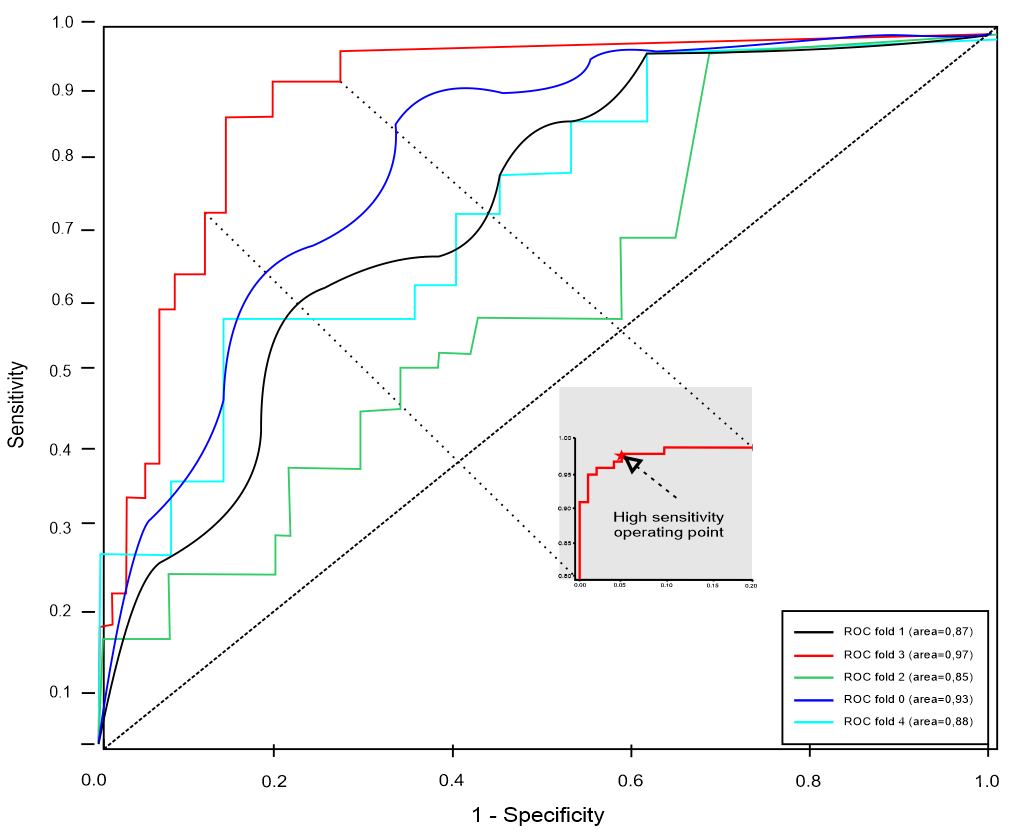
\includegraphics[width=0.9\linewidth]{images/roc_er.png}
		\caption{ER status classification}
        \label{fig:er_roc}
	\end{subfigure}
	\begin{subfigure}{.49\linewidth}
		\centering
		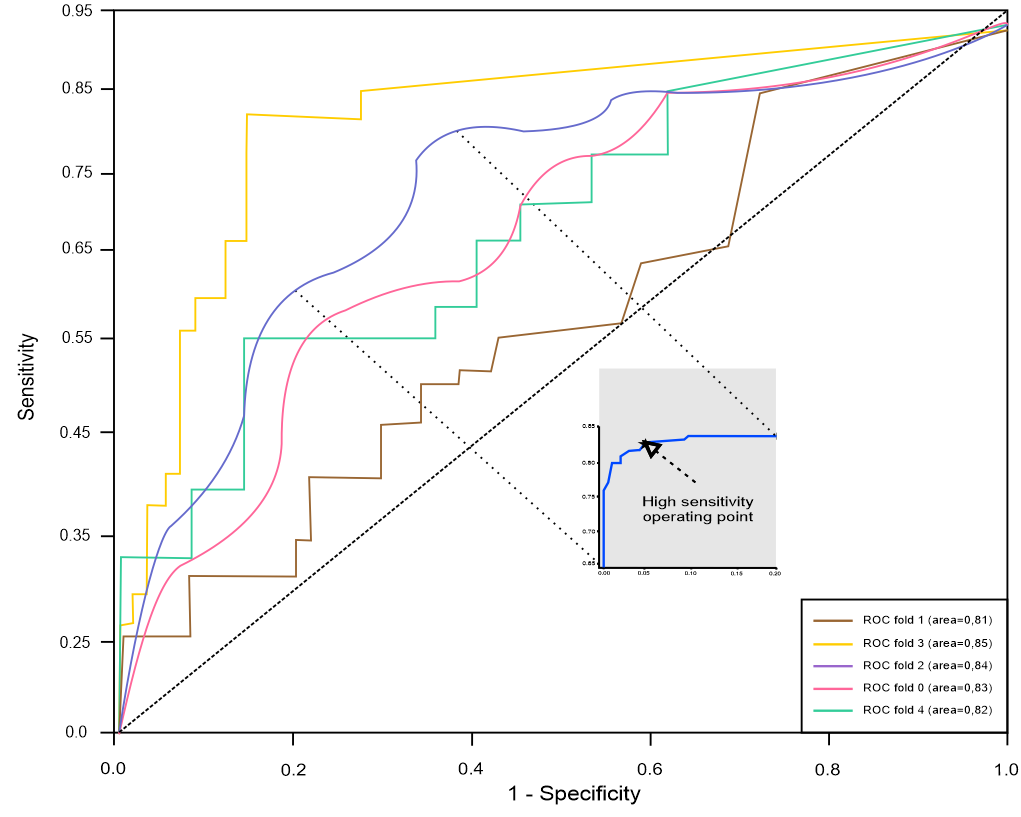
\includegraphics[width=0.9\linewidth]{images/roc_pgr.png}
		\caption{PGR status classification}
        \label{fig:pgr_roc}
	\end{subfigure}\\[1ex]
	\begin{subfigure}{0.49\linewidth}
		\centering
		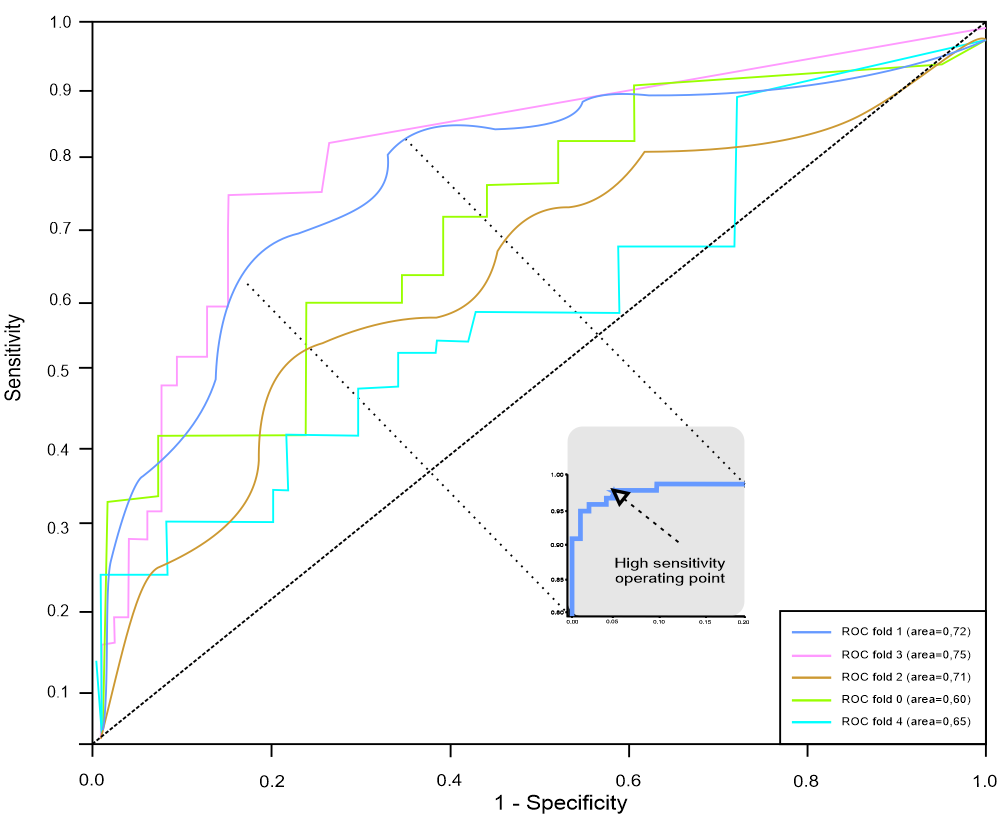
\includegraphics[width=0.9\linewidth]{images/roc_her2.png}
		\caption{HER2 status classification }
        \label{fig:her2_roc}
	\end{subfigure}
	\caption{ROC curve of the best predictor for ER, PGR, and HER2 status classification~\cite{karimACCESS2019}} 
	\label{fig:roc_all}
\end{sidewaysfigure*}
\fi 

\subsection{Analysis of subtype classification}
Results for breast cancer subtype classification based on ER, PGR, and HER2/neu are analysed separately. 

\paragraph{Subtype classification based on ER status} - overall classification results for individual and multimodalities are shown in~\cref{tab:all_results}. As seen, MAE on a combined input of GE and miRNA expression data performs the best compared to any individual input modalities. To provide a view on misclassified instances, confusion matrix is shown in~\cref{fig:er_confusion}. As shown, the MAE model was evaluated on 288 samples, including 197 positive, 55 negative, and 36 indeterminate samples. 

\begin{itemize}[noitemsep]
    \item Out of 197 samples, 187 positive cases were classified correctly, making only 10 mistakes in which 3 were classified as negative and 7 as indeterminate. 

    \item Out of 55 negative cases, 47 were correctly classified, making 8 mistakes in which 3 were classified as positive and 5 as indeterminate. 

    \item Out of 36 indeterminate cases, 25 were correctly classified, making 11 mistakes in which 4 were classified as negative and 7 as positive.  
\end{itemize}

\begin{table}[h]
    \centering
    \footnotesize
    \caption{Top results for ER, PGR, and HER2/neu status classification~\cite{karimACCESS2019}}
    \vspace{-2mm}
    \label{tab:all_results}
    \begin{tabular}{l|l|l|l|l|l} 
        \hline
        \textbf{Tasks} & \textbf{Input modality} & \textbf{MCC} & \textbf{Precision} & \textbf{Recall} & \textbf{F1} \\ 
        \hline
         & DNA methylation   & 0.7573 & 0.8948    & 0.8969 & 0.8958  \\ 
        \cline{2-6}
            & Gene expression  & 0.7745 & 0.8944    & 0.9004 & 0.8964  \\ 
        \cline{2-6}
        ER status       & miRA expression & 0.7235 & 0.8846    & 0.8876 & 0.8857  \\ 
        \cline{2-6}
                      & Gene + miRNA expression  & 0.7928 & 0.9325    & 0.9336 & 0.932   \\ 
        \cline{2-6}
                   & Gene + miRNA expression + DNA methylation & 0.7876 & 0.9175    & 0.918  & 0.9177  \\ 
        \hline
                     & DNA methylation   & 0.6963 & 0.7849    & 0.7939 & 0.7877  \\ 
        \cline{2-6}
                       & Gene expression  & 0.7134 & 0.8166    & 0.8276 & 0.8174  \\ 
        \cline{2-6}
        PGR status  & miRA expression   & 0.7059 & 0.7717    & 0.7743 & 0.7672  \\ 
        \cline{2-6}
                     & Gene + miRNA expression   & 0.7456 & 0.8566    & 0.8633 & 0.856   \\ 
        \cline{2-6}
                     & Gene + miRNA expression + DNA methylation & 0.7791 & 0.7987    & 0.8086 & 0.8001  \\ 
        \hline
                    & DNA methylation   & 0.5632 & 0.376     & 0.613  & 0.466   \\ 
        \cline{2-6}
                     & Gene expression   & 0.5967 & 0.6355    & 0.607  & 0.6173  \\ 
        \cline{2-6}
        HER2/neu status & miRA expression  & 0.6124 & 0.5627    & 0.5885 & 0.5732  \\ 
        \cline{2-6}
                   & Gene + miRNA expression   & 0.6276 & 0.6207    & 0.6444 & 0.627   \\ 
        \cline{2-6}
                   & Gene + miRNA expression + DNA methylation & 0.5743 & 0.3368    & 0.5804 & 0.4263  \\
        \hline
    \end{tabular}
    \vspace{-2mm}
\end{table}

\paragraph{Subtype classification based on PGR status} - overall classification results for individual and multimodalities are shown in~\cref{tab:all_results}, where the best results are highlighted in green. Similar to ER status prediction task, MAE on a combined input of GE and miRNA expression data performed the best compared to any individual input modalities. Other predictors with combined input of DNA methylation + gene expression + miRNA expression also performs relatively well. To provide a view on misclassified instances, confusion matrix is shown in~\cref{fig:pgr_confusion}. As shown, the MAE model was evaluated on 263 samples, including 168 positive, 76 negative, and 21 indeterminate samples. 

\begin{itemize}[noitemsep]
    \item Out of 168 positive cases, 155 were classified correctly, making only 13 mistakes in which only 2 were classified as negative and 11 as indeterminate. 

    \item Out of 19 indeterminate cases, 14 were correctly classified, making 5 mistakes in which 3 were classified as negative and 2 as indeterminate. 

    \item Out of 76 indeterminate cases, 61 were correctly classified, making 15 mistakes in which 10 were classified as positive and 5 as negative.  
\end{itemize}

\begin{figure*}
	\centering
	\begin{subfigure}{.49\linewidth}
		\centering
		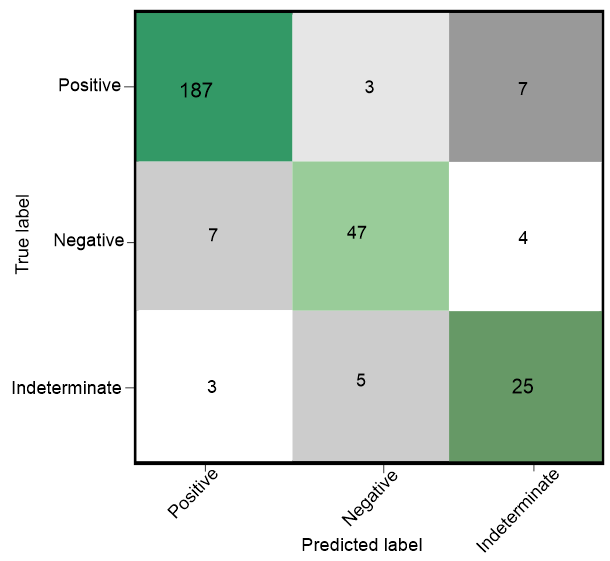
\includegraphics[scale=0.8]{images/conf_er.png}
		\caption{ER status classification}
        \label{fig:er_confusion}
	\end{subfigure}
	\begin{subfigure}{.49\linewidth}
		\centering
		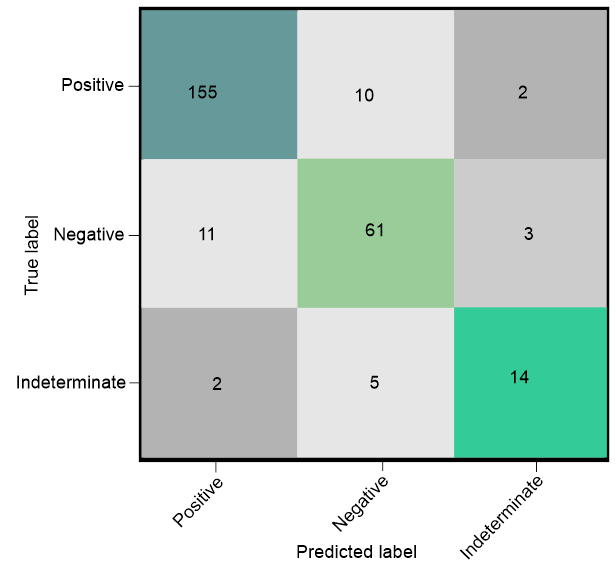
\includegraphics[scale=0.8]{images/conf_pgr.png}
		\caption{PGR status classification}
        \label{fig:pgr_confusion}
	\end{subfigure}
	\begin{subfigure}{0.49\linewidth}
		\centering
		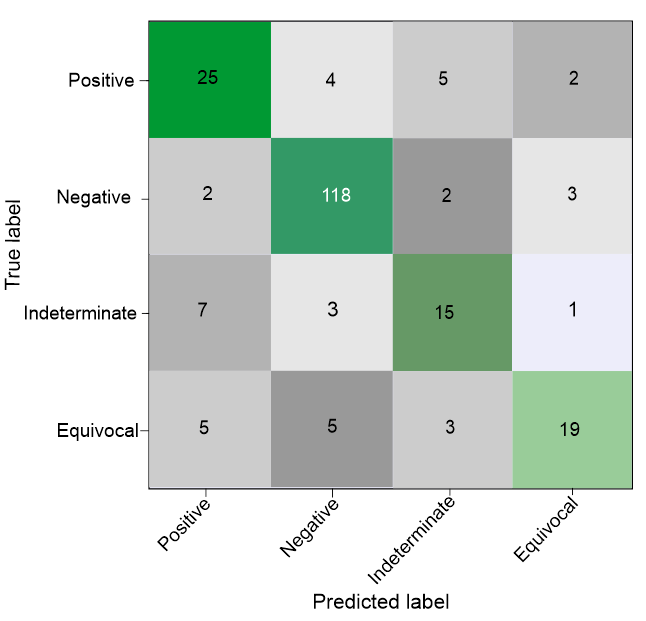
\includegraphics[scale=0.8]{images/conf_her2.png}
		\caption{HER2 status classification }
        \label{fig:her2_confusion}
	\end{subfigure}
	\caption{Confusion matrix for ER, PGR and HER2 status classification~\cite{karimACCESS2019}} 
	\label{fig:multi_cms}
\end{figure*}

\paragraph{Subtype classification based on HER2/neu status} - overall classification results for individual and multimodalities are shown in~\cref{tab:all_results}, where the best results are highlighted in green. Similar to ER and PGR status prediction task, MAE on a combined input of GE and miRNA expression data performed the best compared to any individual input modalities. Other predictors with combined input of DNA methylation + gene expression + miRNA expression also performs relatively well. To provide a view on misclassified instances, confusion matrix is shown in~\cref{fig:her2_confusion}. As shown, the MAE model was evaluated on 219 samples, including 39 positive, 130 negative, 25 indeterminate, and 25 equivocal samples. 

\begin{itemize}[noitemsep]
    \item Out of 39 positive cases, 25 were classified correctly, making 14 mistakes in which 2 were classified as negative, 7 as indeterminate, and 5 as equivocal. 

    \item Out of 130 negative cases, 118 were correctly classified, making 12 mistakes in which 3 were classified as indeterminate, 4 as positive, and 5 as equivocal. 

    \item Out of 25 indeterminate cases, 15 were correctly classified, making 10 mistakes in which 5 were classified as positive, 2 as negative, and 3 as equivocal.
    
    \item Out of 25 equivocal cases, 19 were correctly classified, making 6 mistakes in which 2 were classified as positive, 3 as negative, and 1 as indeterminate.  
\end{itemize}

%\hspace*{3.5mm} The best results for HER2/neu status prediction for each type of input is shown in \cref{tab:all_results}. 

%Similar to ER and PGR status prediction tasks, predictor performs the best with the input of GE data combined with miRNA expression data. However, overall a low accuracy score is observed for each type of data.

%Even after applying several regularization techniques like l2-regularization and Gaussian dropout, result is still poor, which might be because of the overfitting. One of the possible causes for such overfitting is the smaller number of samples~(i.e. 860 samples) compared to ER and PGR statuses~(i.e. 1,024 samples).

%The best result based on gene + miRNA expression modality is highlighted in green in~\cref{tab:all_results}. As shown in confusion matrix in~\cref{fig:her2_confusion}, the predictor is evaluated on 225 samples in which 40 are `HER2/neu Positive', 121 of `HER2/neu Negative', 21 of `HER2/neu Indeterminate', and 32 of are `HER2/neu Equivocal'. The classifier predicted 182 `HER2' cases correctly. Such high mistakes suggests the classifier is probably not yet suitable for clinical setting. %, as it gives 81\% accuracy). 
%Furthermore, the ROC curve of this experiment is shown in~\cref{fig:her2_roc}. As observed, with 2 out of 4 classes achieve lower than 0.5 AUC score: the AUC score for class 0 (`HER2/neu Positive') is 0.83, for class 1 (`HER2/neu Negative') is 0.73, for class 2~(`HER2/neu Indeterminate') is 0.36, and for class 3~(`HER2/neu Indeterminate') is 0.48.

\subsection{Qualitative analysis of learned representation}
Inspired by literature~\cite{rhee2017hybrid} and to qualitatively study whether the learned representation can express biological characteristics of cohorts, t-SNE plots for the latent feature map and the raw GE are depicted in \cref{fig:tnse}. As observed, moderately high distinctive patterns exists between three subtype patients. Since, all the input modality has high dimension, association between each feature is considered. Further, order of subtypes in the t-SNE plot is identical to prognosis of breast cancer subtypes. 

\begin{figure*}
	\centering
	\begin{subfigure}{.48\linewidth}
		\centering
		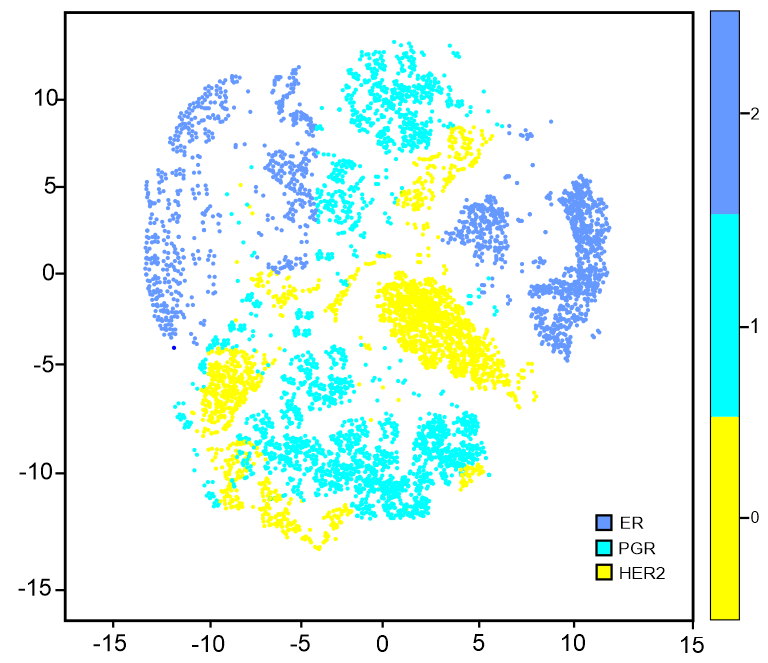
\includegraphics[scale=0.7]{images/raw_tsne.png}
		\caption{t-SNE plot of raw gene expression}
        \label{fig:tsne_raw}
	\end{subfigure}
	\begin{subfigure}{0.48\linewidth}
		\centering
		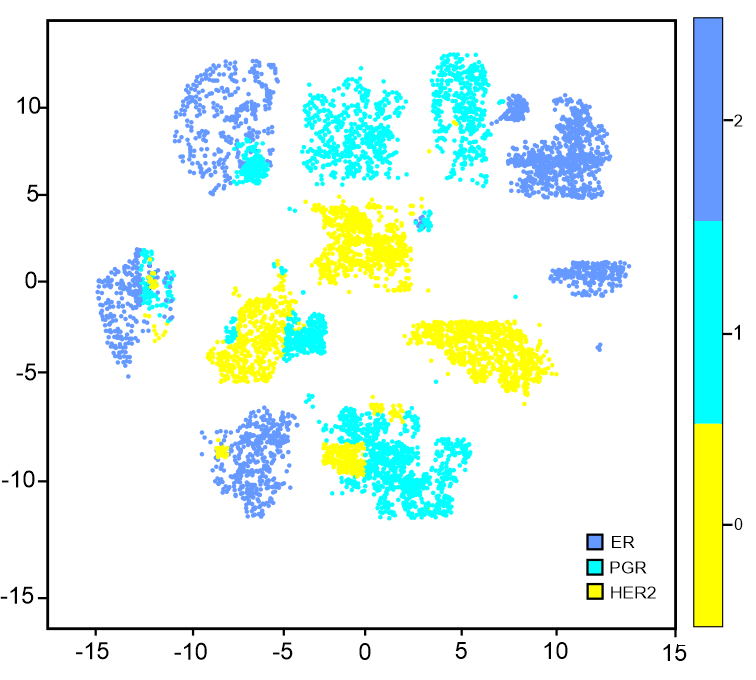
\includegraphics[scale=0.7]{images/ae_tsne.png}
		\caption{t-SNE plot of encoder's latent feature}
        \label{fig:tsne_ae}
	\end{subfigure}
	 \setlength{\belowcaptionskip}{-8pt}
	\caption{t-SNE visualization of gene expressions vs autoencoder latent feature map~\cite{karimACCESS2019}} 
	\label{fig:tnse}
	%\vspace{-2mm}
\end{figure*}

\hspace*{3.5mm} Caruana et al.~\cite{91Caruana} has identified that 80\% of all breast cancers are ER positive in which cancer cells grow in response to the hormone estrogen. On the other hand, about 65\% of these are also PR positive in which the cancer cells grow in response to another hormone, progesterone. ER/PR-positive tumors are much more likely to respond to hormone therapy than tumors that are ER/PR-negative. In about 20\% of breast cancers, cells make too much HER2 protein and tend to be aggressive and fast-growing\footnote{\url{https://www.webmd.com/breast-cancer/}}. In breast cancer, certain subtypes have the worst prognosis e.g. basal, followed by HER2, Luminal B, and Luminal A. The reason is that basal subtype has distinctive molecular characteristics from other subtypes~\cite{bertucci2012basal}. However, all of these patterns are not clearly visible in the raw GE-based t-SNE plots, which signifies that the MAE learned latent molecular properties better from patient expression profiles.

\iffalse
\subsection{Consistency of subtype prognosis}
Inspired from literature~\cite{rhee2017hybrid} and to qualitatively study whether the learned representation can express biological characteristics of the patients, t-SNE of the MAE encoder's output i.e. latent feature map and the t-SNE plot with raw GE are plotted in \cref{fig:tnse}. We can observe moderately high distinctive patterns between three subtype patients. Since, all the input modality has high dimension, we consider the association between each feature. 

\hspace*{3.5mm} Further, we can see that the order of subtypes in the t-SNE plot is identical to prognosis of breast cancer subtypes. Research~\cite{91Caruana} has exposed that 80\% of all breast cancers are ER positive in which the cancer cells grow in response to the hormone estrogen. While about 65\% of these are also PR positive in which the cancer cells grow in response to another hormone, progesterone. ER/PR-positive tumors are much more likely to respond to hormone therapy than tumors that are ER/PR-negative. In about 20\% of breast cancers, the cells make too much HER2 protein and tend to be aggressive and fast-growing\footnote{\url{https://www.webmd.com/breast-cancer/}}. In breast cancer, certain subtype has the worst prognosis e.g. basal, followed by HER2, Luminal B, and Luminal A. The reason is that basal subtype has distinctive molecular characteristics from other subtypes~\cite{bertucci2012basal}. However, not all these patterns clearly visible in the t-SNE plot with raw GE, which signifies that the MAE learned the latent molecular properties better from the patient expression profiles.
\fi 

\subsection{Comparison with ML baselines}
%Although our datasets are collected from TCGA, multimodal features are used to train DL algorithms. Nevertheless, n
None of the related works summarized in~\cref{table:stateofart} used multimodality for breast cancer subtypes. Thus, a one-to-one comparison in a DL setting was not viable. Therefore, ML baseline models classifiers created based on both unimodal and multimodal inputs. In particular, support vector machines~(SVM), Na{\"i}ve Bayes~(NB), logistic regression~(LR), k-nearest neighbors algorithm~(KNN), decision trees~(DT), random forest~(RF), and gradient boosted trees~(GBT). In this setting, hyperparameter optimization is performed using random search with 5-fold cross validation. 

\begin{table*}
	\renewcommand{\arraystretch}{0.9}
	\caption{Subtypes prediction with ML classifiers~(*=modality with best results)~\cite{karimACCESS2019}}
	\label{table:classification}
	\vspace{-2mm}
	\scriptsize
	\centering
	\begin{tabular}{p{2.5cm}|l|r|r|r}
		\toprule
		\textbf{Modality} & \textbf{Classifier} & \textbf{Precision} & \textbf{Recall} & \textbf{MCC}\\ \hline
		\multirow{7}{*}{DM} & LR & 0.74 & 0.72 & 0.53 \\
		& NB & 0.73 & 0.70 & 0.55 \\
		& SVM & 0.80 & 0.81 & 0.69 \\
		& KNN & 0.69 & 0.71 & 0.51 \\
		& GBT & 0.88 & 0.85 & 0.72\\
		& RF & 0.91 & 0.92 & 0.75\\
		& \textbf{MAE}  & 0.93 & 0.91 & 0.79 \\
		\hline
		\multirow{7}{*}{GE} & LR & 0.76 & 0.72 & 0.59 \\
		& NB & 0.73 & 0.72 & 0.55 \\
		& SVM & 0.80 & 0.81 & 0.66 \\
		& KNN & 0.73 & 0.73 & 0.53 \\
		& GBT & 0.87 & 0.86 & 0.74\\
		& RF & 0.89 & 0.88 & 0.77\\
		& \textbf{MAE} & 0.92 & 0.91 & 0.79 \\ 
		\hline
		\multirow{7}{*}{miRNA} & LR & 0.75 & 0.73 & 0.54 \\
		& NB & 0.72 & 0.71 & 0.53 \\
		& SVM & 0.78 & 0.79 & 0.68 \\
		& KNN & 0.71 & 0.69 & 0.53 \\
		& GBT & 0.87 & 0.85 & 0.71\\
		& RF & 0.89 & 0.86 & 0.73\\
		& \textbf{MAE} & 0.89 & 0.90 & 0.75 \\ 
		\hline
		\multirow{7}{*}{GE+miRNA*} & LR & 0.72 & 0.71 & 0.57 \\
		& NB & 0.69 & 0.70 & 0.51 \\
		& SVM & 0.75 & 0.74 & 0.64 \\
		& KNN & 0.63 & 0.59 & 0.49 \\
		& GBT & 0.83 & 0.82 & 0.69\\
		& RF & 0.84 & 0.85 & 0.71\\
		& \textbf{MAE} & 0.87 & 0.88 & 0.74 \\ 
		\hline
		\multirow{7}{*}{DM+GE+miRNA} & LR & 0.65 & 0.68 & 0.47 \\
		& NB & 0.70 & 0.71 & 0.50 \\
		& SVM & 0.72 & 0.73 & 0.55 \\
		& KNN & 0.69 & 0.66 & 0.52 \\
		& GBT & 0.81 & 0.82 & 0.65\\
		& RF & 0.82 & 0.83 & 0.66\\
		& \textbf{MAE} & 0.84 & 0.85 & 0.69 \\
        \hline
	\end{tabular}
\end{table*}

\hspace*{3.5mm} As shown in \cref{table:classification}, GBT and RF classifiers perform consistently better for subtype classification. This finding is further validated by calibrating the best performing MAE classifier for which the output probability of the classifier can be directly interpreted as a confidence level in terms of `fraction of positives'~(FOP). MAE classifier gave a probability value~(i.e. FOP) between 0.82 to 0.93. This signifies that 93\% of the predictions belong to true positives, whereas the second best GBT and RF generates the FOP values between 0.75 to 0.87 and between 0.76 to 0.89, respectively. 

\section{Discussion}\label{chapter_4:discussion}
The MAE implementation based on GE and miRNA expression modalities gave the best result for breast cancer subtypes classification, covering both ER, PGR, and HER2 status. This is also the best for individual classification tasks. On the other hand, HER2 status classification got the worst results by far compared to ER and PGR status ones. One potential reason is that HER2 status data has fewer samples compared to ER and PGR ones. Besides, both training and validation accuracies for each classifier far exceeds compared to test accuracy, which is probably because of overfitting. This is justifiable as we lack of enough  training samples. As shown in~\cref{fig6}, the number of samples across datasets is only 1,000. While, the smallest number of feature~(e.g. 1,881 features in miRNA expression) still exceeds it, where the number of features in DNA methylation and GE exceeds other modalities. 

\begin{figure*}
	\centering
	\begin{subfigure}{.49\linewidth}
		\centering
		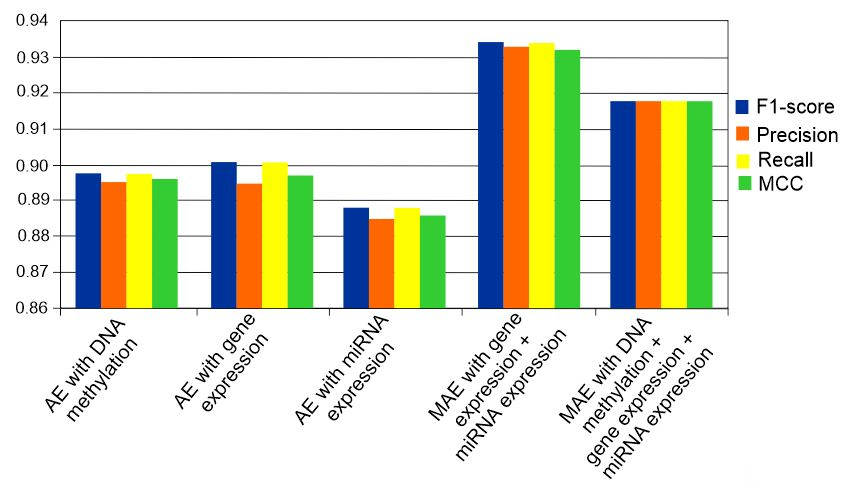
\includegraphics[scale=0.8]{images/1.png}
		\caption{ER status classification}
        \label{fig:top_er}
	\end{subfigure}
	\begin{subfigure}{.49\linewidth}
		\centering
		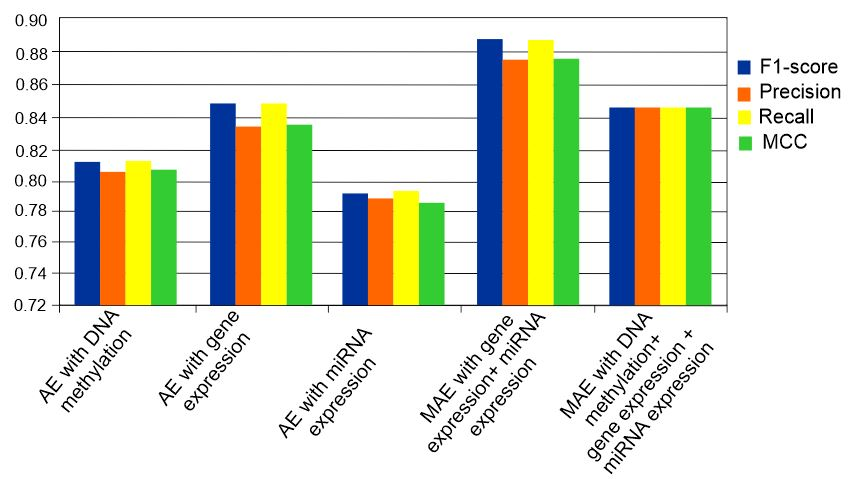
\includegraphics[scale=0.8]{images/2.png}
		\caption{PGR status classification}
        \label{fig:top_pgr}
	\end{subfigure}
	\begin{subfigure}{0.49\linewidth}
		\centering
		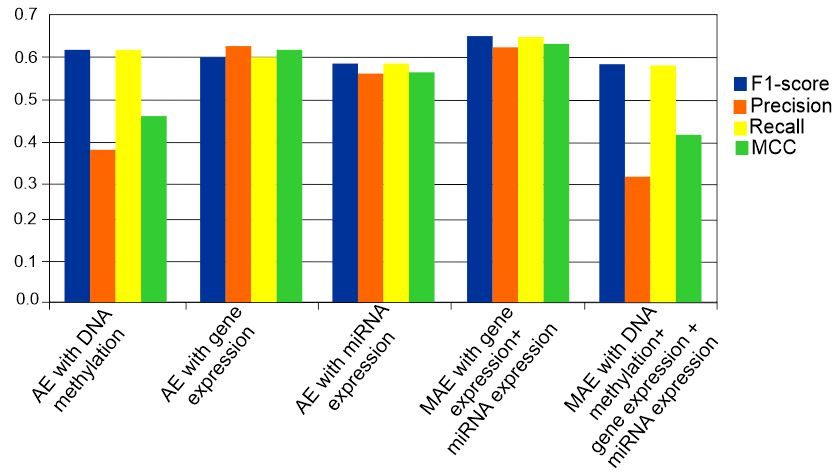
\includegraphics[scale=0.8]{images/3.png}
		\caption{HER2 status classification }
        \label{fig:top_her2}
	\end{subfigure}
	\caption{Top ER, PGR, and HER2 status classifications results for each input type~\cite{karimACCESS2019}} 
	\label{fig6}
		\vspace{-2mm} 
\end{figure*}

\hspace*{3.5mm} Among ML baselines, both validation and training scores for SVM model converge to a low value with increasing size of the training set. Consequently, SVM did not benefit much from more training samples. However, being tree-based ensemble methods RF and GBT models can learn more complex concepts from GE + miRNA multimodal features, similar to MAE. The reason is that both RF and GBT models contributes to higher variance and lowering the bias. This is observed from higher training scores compared to validation scores for the maximum number of samples i.e. adding more training samples does increase model generalization. Overall, MAE gave relatively better results compared to regular AE with a single type of input. 
%as well as other best ML baselines, e.g., GBT and RF. 
It mostly occurs with the GE + miRNA expression giving the best results for subtypes classification.
%and decent results for survival rate prediction. 
Based on this comparison, we can evidently conclude that MAE outperforms both AE and ML baselines models, with the right combination of inputs.

\hspace*{3.5mm} Although, the best result for every status classification was recorded by MAE based on GE + miRNA expression input modality, MAE model also made non-trivial mistakes, specially for the HER2/neu-based subtype classification tasks. Such high mistakes made the classifier not yet suitable for real clinical setting. To diagnose and mitigate the high misclassification error, several regularization techniques such as l2-regularization and Gaussian dropout were employed. However, still poor was observed, which might be due to overfitting of the network. One of the possible causes for such overfitting is the smaller number of samples~(i.e. 860 samples) compared to ER and PGR statuses~(i.e. 1,024 samples). 

\section{Chapter Summary}\label{chapter_4:conclusion}
In this chapter, a DSS is developed for predicting different subtypes of breast cancer patients, which is technically based on an multimodal autoencoder architecture. An F1-score of 0.93 and 0.856 were observed for ER and PGR-based diagnosis, respectively with GE and miRNA expression input modality. On the other hand, with an F1 score of 0.627, HER2 status classification got the worst results by far compared to ER and PGR status ones. Although some results looks promising, overall decision accuracy of the DSS is hindered due to several factors. The key findings of this chapter can summarised as follows: 

\begin{enumerate}[noitemsep]
    \item Limited availability of genomics data, which is probably due to individual patients privacy. Besides, sources like ICGC and COSMIC are not comprehensive even requiring restricted access. Limited amount of labeled data was one of the main reasons caused the MAE classifiers overfitted. 
    
    \item Adding more training samples helped increase model's generalization capability. This suggest that the prediction can be made more confidently on more labelled training data. 
    
    \item No manual feature engineering and selection were performed. Rather, the multimodal representation learning strategy let the network to choose the best features from the very high dimensional inputs. Consequently, pretraining loss for some input combinations were getting out of bound. 

    \item The best result observed with GE + miRNA expression  multimodality suggest that DNA methylation is not very suitable for none of the subtypes classification tasks. The worst results for HER2 status classification suggest that none of the input modalities are suitable for the clinical diagnosis. 
    
    \item The DSS based on multimodal data is black-box, hence lack of interpretability. Besides, high classification mistakes suggest that even the best model yet not suitable for real clinical setting.
\end{enumerate}

\hspace*{3.5mm} In the next chapter, we extend both single and multimodality-based cancer typing methods to overcome above mentioned limitations. We will increase the training data, by combining samples from the Pan Cancer Atlas project. We will focus on improving the explanations of the predictions using different probing techniques.
Class-specific heat maps will be generated using guided-gradient class activation maps++~(Grad-CAM++)~\cite{chattopadhay2018grad} and layer-wise relevance propagation~(LRP)~\cite{LRP3}, to identify significant biomarkers.To provide both global and local interpretation: i) import biomarkers will be identified based on feature importance, followed by ranking top genes across all the cancer types, ii) we sensitivity analysis and feature interactions will be discussed to explain individual diagnosis decision. 
